\begin{questions}
\question{
	In un'azienda sono disponibili tre auto aziendali destinate agli spostamenti di lavoro. L'assegnamento avviene attraverso la firma di un documento da parte del soggetto che le utilizza, diventando così unico responsabile dell'auto assegnata. Le quattro figure autorizzate al loro impiego hanno ruoli e responsabilità specifici che determinano la priorità nell'utilizzo dei veicoli.
	\begin{itemize}
		\item Amministratore delegato (A)
		\item Manager (M)
		\item Venditore (V)
		\item Stagista (S)
	\end{itemize}
	
	Si chiede di progettare un sistema automatico per la presa in carico delle automobili, considerando che tutte le figure potrebbero avere tale necessità in contemporanea, considerando il seguente ordine di priorità: A $>$ M $>$ V $>$ S.



  Il sistema di accesso è gestito tramite 4 differenti variabili ``C'', ``D'', ``E'' e ``F'' secondo la codifica riportata in Tabella \ref{tab:codifica}.

    \begin{table}[h!]
        \centering
            \begin{tabular}{ |p{1cm}|p{1cm} |p{1cm}|p{1cm}| p{5cm}|  }
                 \hline
                 \multicolumn{5}{|c|}{Codifica assegnazione auto} \\
                 \hline
                 C & D & E & F & Codice\\
                 \hline
                 0 & 0 & 0 & 0 & Nessun assegnamento\\
                 1 & 0 & 0 & 0 & A\\
                 0 & 1 & 0 & 0 & M\\
                 0 & 0 & 1 & 0 & V\\
                 0 & 0 & 0 & 1 & S\\
                 1 & 1 & 0 & 0 & AM\\
                 1 & 0 & 1 & 0 & AV\\
                 1 & 0 & 0 & 1 & AS\\
                 0 & 1 & 1 & 0 & MV\\
                 0 & 1 & 0 & 1 & MS\\
                 0 & 0 & 1 & 1 & VS\\
                 1 & 1 & 1 & 0 & AMV\\
                 1 & 1 & 0 & 1 & AMS\\
                 1 & 0 & 1 & 1 & AVS\\
                 0 & 1 & 1 & 1 & MVS\\
                 \hline
            \end{tabular}

        \label{tab:codifica}
    \end{table}

}

\newpage
    \begin{solution}
       \mysection{Formulazione}
        Creazione della tabella di verità.
        
            \begin{center}
              \begin{tabular}{cccc|cccc|c}
                A & M & V & S 	& F & E & D & C & Assegnamento\\
                \hline
                0 & 0 & 0 & 0 	& 0 & 0 & 0 & 0 & Nessuno\\
                0 & 0 & 0 & 1 	& 1 & 0 & 0 & 0 & S\\
                0 & 0 & 1 & 0 	& 0 & 1 & 0 & 0 & V\\
                0 & 0 & 1 & 1 	& 1 & 1 & 0 & 0 & VS\\
                0 & 1 & 0 & 0 	& 0 & 0 & 1 & 0 & M\\ 
                0 & 1 & 0 & 1 	& 1 & 0 & 1 & 0 & MS\\
                0 & 1 & 1 & 0 	& 0 & 1 & 1 & 0 & MV\\
                0 & 1 & 1 & 1 	& 1 & 1 & 1 & 0 & MVS\\
                1 & 0 & 0 & 0 	& 0 & 0 & 0 & 1 & A\\
                1 & 0 & 0 & 1 	& 1 & 0 & 0 & 1 & AS\\
                1 & 0 & 1 & 0 	& 0 & 1 & 0 & 1 & AV\\
                1 & 0 & 1 & 1 	& 1 & 1 & 0 & 1 & AVS\\
                1 & 1 & 0 & 0 	& 0 & 0 & 1 & 1 & AM\\
                1 & 1 & 0 & 1 	& 1 & 0 & 1 & 1 & AMS\\
                1 & 1 & 1 & 0 	& 0 & 1 & 1 & 1 & AMV\\
                1 & 1 & 1 & 1 	& 0 & 1 & 1 & 1 & AMV\\
              \end{tabular}
            \end{center}
            
        \vspace{-1em}
            
        \mysection{Ottimizzazione}
            Creazione delle Mappe di Karnaugh.
            \begin{enumerate}
                    \item Mappa di Karnaugh per F.
                    
                        \begin{center}
                            \begin{karnaugh-map}[4][4][1][$VS$][$AM$]
                                \manualterms{
                                	0,1,0,1,
                                	0,1,0,1,
                                	0,1,0,1,
                                	0,1,0,0}
                                \implicant{1}{7}
                                \implicant{1}{9}
                                \implicantedge{1}{3}{9}{11}
                             \end{karnaugh-map}
                        \end{center}
                        \[ F = \overline{V}S  +  \overline{A}S + \overline{M}S  \]
                    

                    \item Mappa di Karnaugh per E.
                    
                        \begin{center}
                            \begin{karnaugh-map}[4][4][1][$VS$][$AM$]
                                \manualterms{                  0,0,1,1,
                                	0,0,1,1,
                                	0,0,1,1,
                                	0,0,1,1}
                                \implicant{3}{10}
                             \end{karnaugh-map}
                        \end{center}
                    \[ E = V \]
             

                    \item Mappa di Karnaugh per D.
                    
                        \begin{center}
                            \begin{karnaugh-map}[4][4][1][$VS$][$AM$]
                                \manualterms{                  0,0,0,0,
									1,1,1,1,
									0,0,0,0,
									1,1,1,1}
                                \implicant{4}{14}
                             \end{karnaugh-map}
                        \end{center}
                    \[ D = M \]
                    
                    \newpage
              
                    \item Mappa di Karnaugh per C.
                    
	                    \begin{center}
	                    	\begin{karnaugh-map}[4][4][1][$VS$][$AM$]
	                    		\manualterms{                  0,0,0,0,
	                    			0,0,0,0,
	                    			1,1,1,1,
	                    			1,1,1,1}
	                    		\implicant{12}{10}
	                    	\end{karnaugh-map}
	                    \end{center}
	                    \[ C = A \]
                    
                    
            \end{enumerate}
            
            \mysection{Disegno del circuito}
            Disegno del circuito combinatorio non minimizzato.

            \begin{center}
                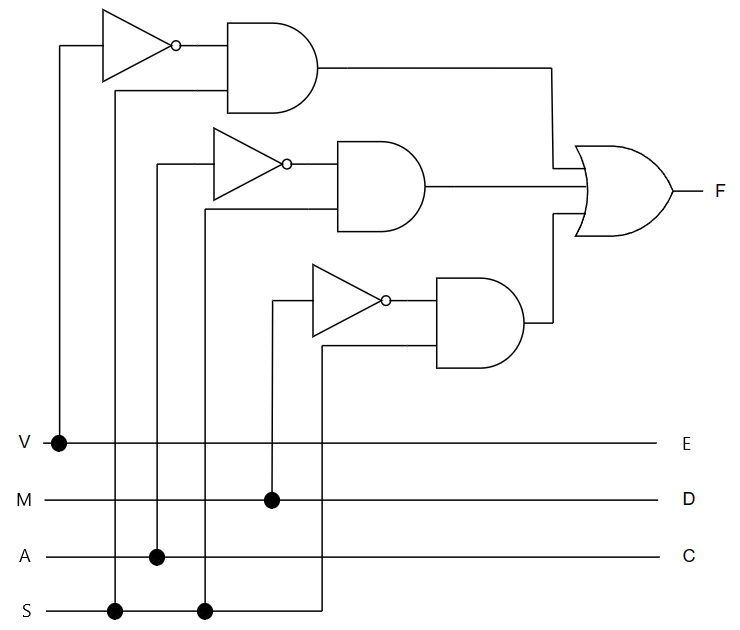
\includegraphics[width=13cm, keepaspectratio]{img/circuito.png}
            \end{center}
            
            \newpage
            
            Le formule usate nella realizzazione del circuito combinatorio sono risultate essere già minimizzate quindi abbiamo cercato di lavorare sull'utilizzo di porte logiche equivalenti ma che ci permettessero di risparmiare sulle componenti. Alla fine, siamo arrivati inizialmente al seguente risultato...
            
            \begin{center}
				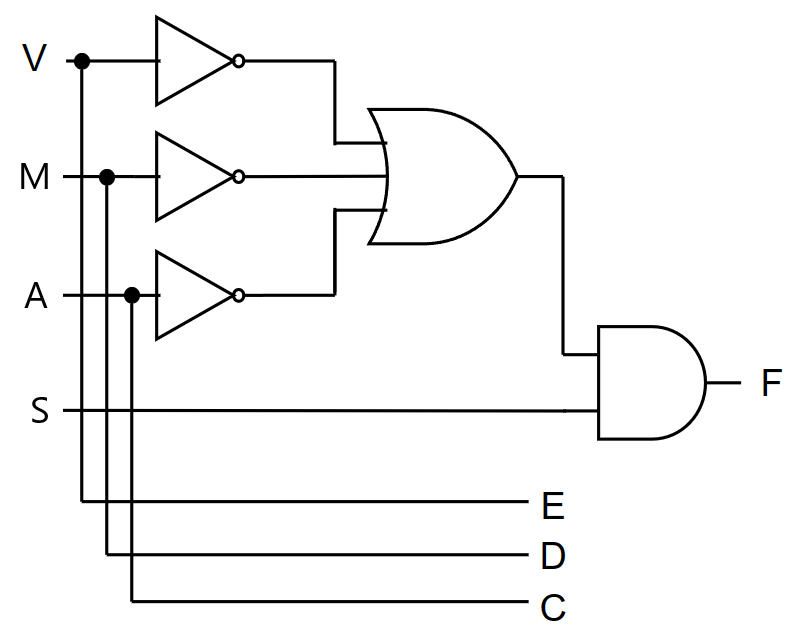
\includegraphics[width=9cm, keepaspectratio]{img/circuito_minimizzato_1.png}
            \end{center}
            
            ... per poi accorgerci che poteva essere minimizzato ulteriormente nel seguente:
            
            \begin{center}
            	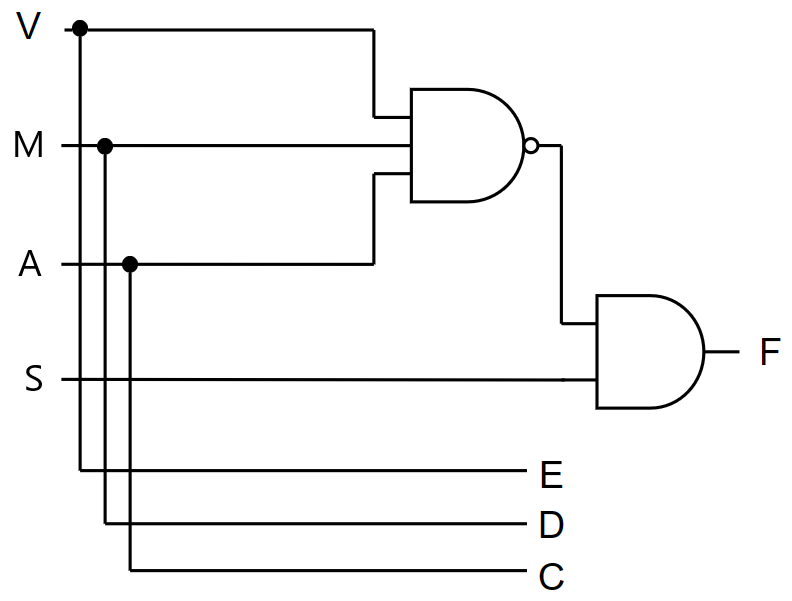
\includegraphics[width=9cm, keepaspectratio]{img/circuito_minimizzato_2.png}
            \end{center}
                 

    \end{solution}
\end{questions}